\documentclass{beamer}
\usepackage[utf 8]{inputenc}
\usepackage[T1]{fontenc}
\usepackage[catalan,english]{babel}
\usepackage{amsmath}
\usepackage{amssymb}
\usepackage{amsthm}
\usepackage{graphicx}
\usepackage{subcaption}
\usepackage{tikz}
\usepackage{upgreek}
\usepackage{multirow}

\mode<presentation>{
\usetheme{Boadilla}
\usecolortheme{seahorse}
}

\title[Sistema termoel\`{e}ctric a la nanoscala]{{\textbf{Modelitzaci\'{o} d'un sistema termoel\`{e}ctric a la nanoscala a trav\'{e}s d'una equaci\'{o} hidrodin\`{a}mica}}}
\author[Alejandro Plaza Gall\'{a}n]{\huge{Alejandro Plaza Gall\'{a}n}\\\vspace{2mm}\Large{Supervisat per: F. Xavier \'{A}lvarez Calafell\\ i Albert Beardo Ricol}\vspace{-0.5cm}}
\date{Setembre de 2021}

\begin{document}

\begin{frame}
\titlepage
\centering
\includegraphics[width=0.30\textwidth]{../grafics/logo-uab.png}\par\vspace{1cm}
\end{frame}

\begin{frame}{Introducci\'{o}}
\begin{itemize}
\item Els components dels aparells electr\`{o}nics s\'{o}n cada cop m\'{e}s petits
\pause
\vspace{5mm}
\item Aix\`{o} augmenta la calor produ\"{i}da
\pause
\vspace{5mm}
\item S'han de buscar maneres de dissipar la calor
\pause
\vspace{5mm}
\item La llei de Fourier \'{e}s l'equaci\'{o} cl\`{a}ssica per la conducci\'{o} de la calor
\pause
\vspace{5mm}
\item A la nanoscala es necessita un nou model: el model hidrodin\`{a}mic
\end{itemize}
\end{frame}

\begin{frame}{Objectius}
\begin{itemize}
\item Objectiu principal: dissenyar un invent tecnol\`{o}gic per disminuir la temperatura dels components electr\`{o}nics
\pause
\vspace{5mm}
\item Per all\`{o}:
\vspace{5mm}
\begin{itemize}
\item Comparar els dos models amb dades experimentals
\pause
\vspace{5mm}
\item Fer simulacions per veure la necessitat del model hidrodin\`{a}mic
\pause
\vspace{5mm}
\item Simular un conductor escalfat sobre un substrat de silici
\pause
\vspace{5mm}
\item Afegir-hi un l\`{a}ser per refredar-lo
\end{itemize}
\end{itemize}
\end{frame}

\begin{frame}{Llei de Fourier}

\tikzset{every picture/.style={line width=0.75pt}}
\begin{figure}
\begin{center}
\begin{tikzpicture}[x=0.75pt,y=0.75pt,yscale=-0.6,xscale=0.6]
\draw (212.5,134) .. controls (219.43,108.41) and (253.94,87.36) .. (289.5,72.99) .. controls (320.63,60.4) and (352.56,52.93) .. (367.5,52);
\draw (212.5,134) .. controls (257.5,159) and (285.5,224) .. (284.5,269);
\draw (284.5,269) .. controls (297.5,221) and (407.5,189) .. (439.5,187);
\draw (367.5,52) .. controls (412.5,77) and (440.5,142) .. (439.5,187);
\draw (315.5,63) .. controls (360.5,88) and (388.5,153) .. (387.5,198);
\draw (261.5,86) .. controls (306.5,111) and (334.5,176) .. (333.5,221);
\draw (249.5,167) .. controls (256.43,141.41) and (290.94,120.36) .. (326.5,105.99) .. controls (357.63,93.4) and (389.56,85.93) .. (404.5,85);
\draw (276.5,219) .. controls (283.43,193.41) and (317.94,172.36) .. (353.5,157.99) .. controls (384.63,145.4) and (416.56,137.93) .. (431.5,137);
\draw (389.5,113) -- (465.11,34.44);
\draw[shift={(466.5,33)},rotate=493.91][color={rgb,255:red,0;green,0;blue,0}][line width=0.75] (10.93,-3.29) .. controls (6.95,-1.4) and (3.31,-0.3) .. (0,0) .. controls (3.31,0.3) and (6.95,1.4) .. (10.93,3.29);
\draw (326.5,97) -- (402.11,18.44);
\draw[shift={(403.5,17)},rotate=493.91][color={rgb,255:red,0;green,0;blue,0}][line width=0.75] (10.93,-3.29) .. controls (6.95,-1.4) and (3.31,-0.3) .. (0,0) .. controls (3.31,0.3) and (6.95,1.4) .. (10.93,3.29);
\draw (402.5,183) -- (478.11,104.44);
\draw[shift={(479.5,103)},rotate=493.91][color={rgb,255:red,0;green,0;blue,0}][line width=0.75] (10.93,-3.29) .. controls (6.95,-1.4) and (3.31,-0.3) .. (0,0) .. controls (3.31,0.3) and (6.95,1.4) .. (10.93,3.29);
\draw (256.5,120) -- (332.11,41.44);
\draw[shift={(333.5,40)},rotate=493.91][color={rgb,255:red,0;green,0;blue,0}][line width=0.75] (10.93,-3.29) .. controls (6.95,-1.4) and (3.31,-0.3) .. (0,0) .. controls (3.31,0.3) and (6.95,1.4) .. (10.93,3.29);
\draw (300.5,205) -- (376.11,126.44);
\draw[shift={(377.5,125)},rotate=493.91][color={rgb,255:red,0;green,0;blue,0}][line width=0.75] (10.93,-3.29) .. controls (6.95,-1.4) and (3.31,-0.3) .. (0,0) .. controls (3.31,0.3) and (6.95,1.4) .. (10.93,3.29);

\draw (472,28) node[anchor=north west][inner sep=0.75pt][font=\Huge][align=left] {$\boldsymbol{q}$};
\draw (178,107) node[anchor=north west][inner sep=0.75pt][font=\huge][align=left] {$S$};
\end{tikzpicture}

\end{center}
\end{figure}
\pause
Equaci\'{o} de la llei de Fourier:
\[\boldsymbol{q}=-\kappa\nabla T\]
\pause
\vspace{-6mm}
\begin{itemize}
\item $\boldsymbol{q}$: flux de calor
\pause
\item $T$: temperatura
\pause
\item $\kappa$: conductivitat t\`{e}rmica
\end{itemize}
\end{frame}

%\begin{frame}{Llei de Fourier}
%Equaci\'{o} de conservaci\'{o} de l'energia:
%\[\rho c_e\dot{T}+\nabla\cdot\boldsymbol{q}=Q,\]
%\pause
%
%on $\rho$ \'{e}s la densitat,
%\pause
%
%$c_e$ \'{e}s la calor espec\'{i}fica,
%\pause
%
%$Q$ \'{e}s la densitat de la font de calor.
%\pause
%\vspace{3mm}
%
%Nom\'{e}s estudiarem estats estacionaris, pels quals les derivades temporals seran 0.
%\pause
%
%Per tant no caldran condicions inicials, nom\'{e}s condicions de contorn.
%\end{frame}
%
\begin{frame}{Model hidrodin\`{a}mic}
Equaci\'{o} hidrodin\`{a}mica:
\[\tau\dot{\boldsymbol{q}}+\boldsymbol{q}=-\kappa\nabla T+\ell^2\big(\nabla^2\boldsymbol{q}+2\nabla(\nabla\cdot\boldsymbol{q})\big)\]
\pause
\begin{itemize}
\item $\tau$: temps de relaxaci\'{o} del flux
\pause
\item $\ell$: dist\`{a}ncia no local
\end{itemize}
\pause
\vspace{4mm}

%Aquests par\`{a}metres s\'{o}n intr\'{i}nsecs, \'{e}s a dir, no depenen de la geometria del sistema.
%
A grans escales, $\tau$ i $\ell$ es tornen negligibles i recuperem la llei de Fourier
\end{frame}


\begin{frame}{L\`{a}mina fina de silici}
\vspace{-6mm}
\begin{figure}
\begin{center}
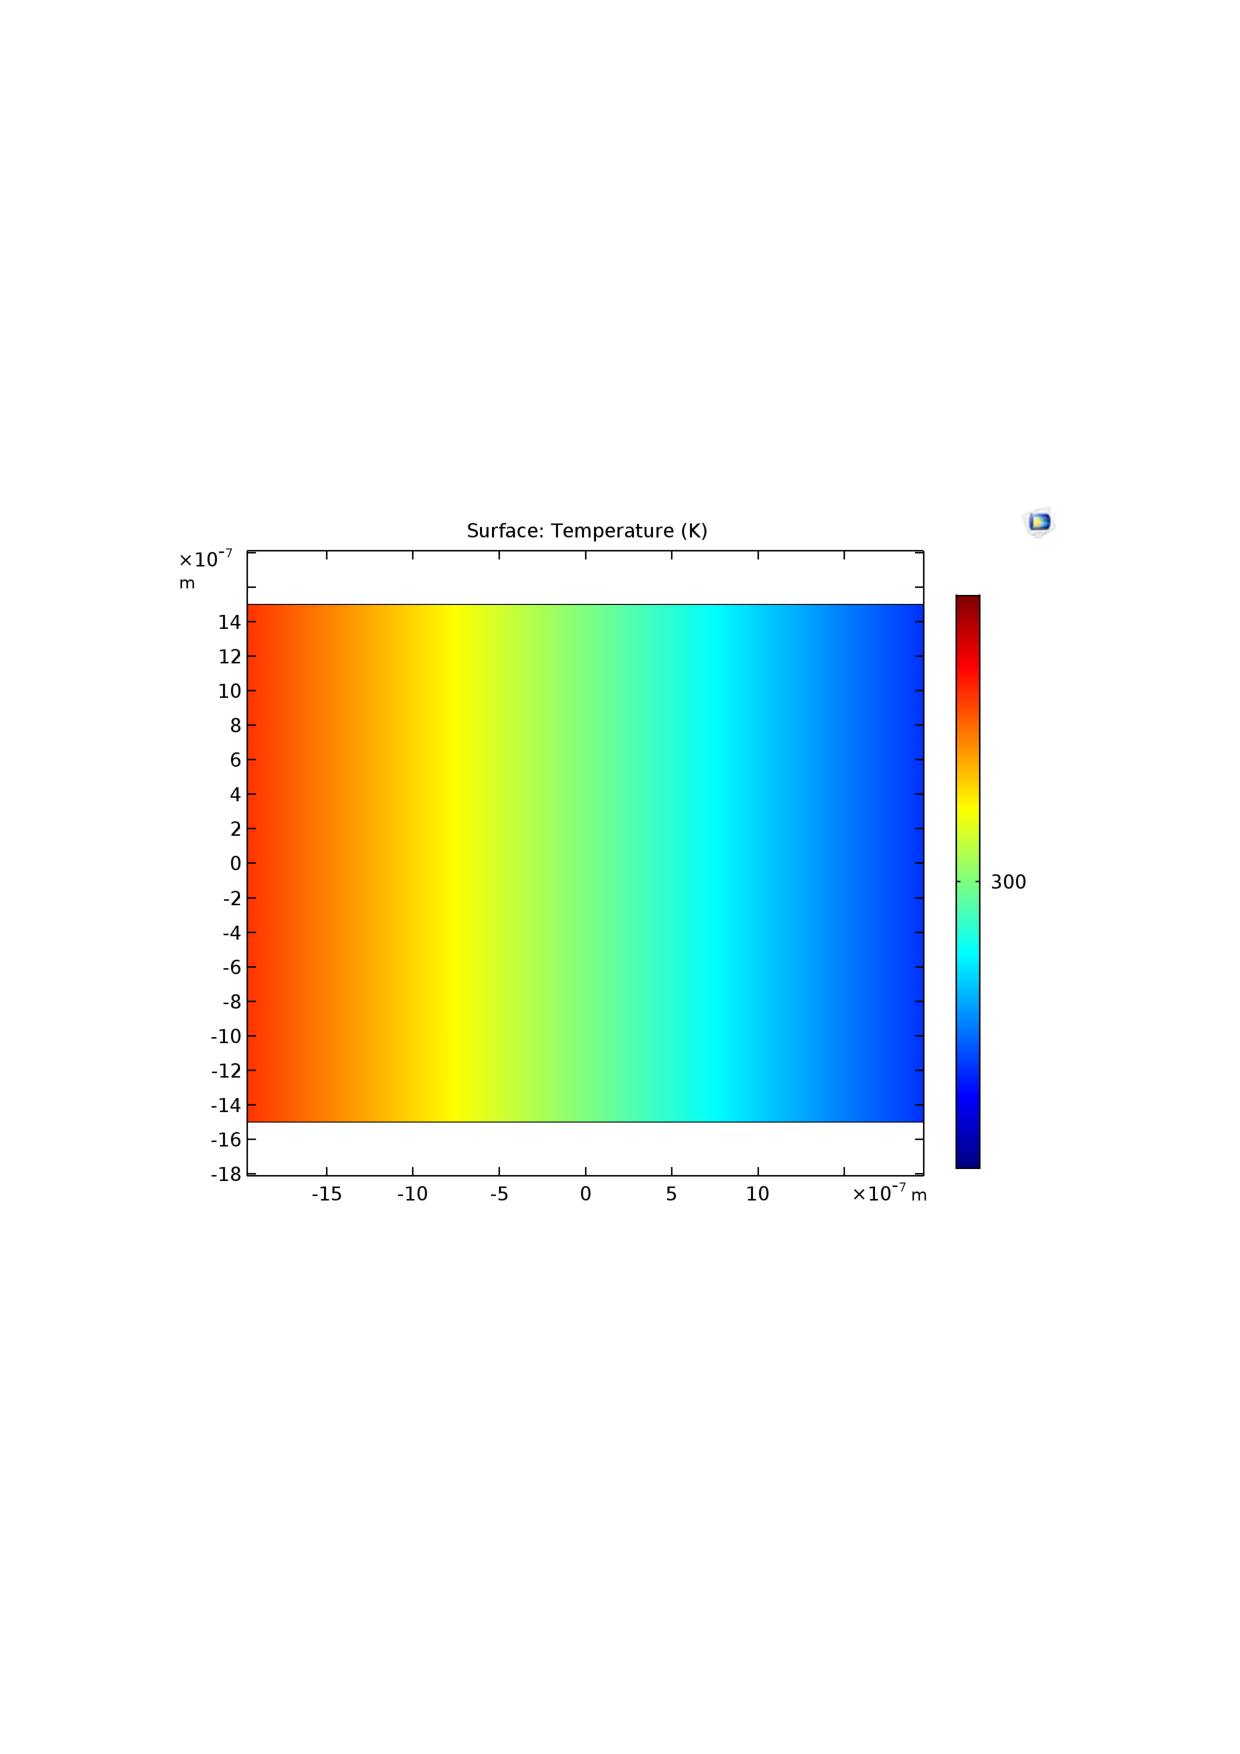
\includegraphics[scale=0.45]{../grafics/film/tf-temperatura.pdf}
\end{center}
\end{figure}
\vspace{-4mm}
\begin{itemize}
\item Simulem una secci\'{o} d'una fina l\`{a}mina de silici
\pause
\item Gradient de temperatures horitzontal
\pause
\item Condicions de contorn:
\begin{itemize}
\item Paret esquerra: 300,5 K
\pause
\item Paret dreta: 299,5 K
\end{itemize}
\end{itemize}
\end{frame}

\begin{frame}{L\`{a}mina fina de silici}
\begin{figure}
\begin{center}
\vspace{-4mm}
Perfil del flux de calor respecte la posici\'{o} $y$ segons:
\begin{subfigure}{0.49\textwidth}
\begin{itemize}
\item Fourier (morat)
\item Hidrodin\`{a}mic (verd)
\item Fourier amb $\kappa_{\text{eff}}$ (blau)
\end{itemize}
\end{subfigure}
\begin{subfigure}{0.49\textwidth}
\caption*{$H=3$ $\upmu$m}
\vspace{-2mm}
\includegraphics[scale=0.235]{../grafics/film/3-mum.png}
\end{subfigure}
\begin{subfigure}{0.49\textwidth}
\caption*{$H=$ 1,6 $\upmu$m}
\vspace{-2mm}
\includegraphics[scale=0.235]{../grafics/film/1-6-mum.png}
\end{subfigure}
\begin{subfigure}{0.49\textwidth}
\caption*{$H=$ 0,42 $\upmu$m}
\vspace{-2mm}
\includegraphics[scale=0.235]{../grafics/film/0-42-mum.png}
\end{subfigure}
\end{center}
\end{figure}
\end{frame}

\begin{frame}{L\`{a}mina fina de silici}
Conductivitat t\`{e}rmica del silici: $150$ W/mK
\begin{table}[ht!]
\centering
\label{Tab:keff}
\begin{tabular}{c|c|c}
\multirow{3}{*}{$\boldsymbol{H}$ \textbf{(}$\boldsymbol{\upmu}$\textbf{m)}}&$\boldsymbol{\kappa}_{\text{\textbf{eff}}}$ \textbf{calculada (W/mK)}&$\boldsymbol{\kappa}_{\text{\textbf{eff}}}$ \textbf{experimental (W/mK)}\vspace{-0.7mm}\\
&\multirow{2}{*}{\footnotesize{(presa de la simulaci\'{o})}}&\footnotesize{(presa de Beardo \emph{et al.}}\vspace{-0.7mm}\\
&&\footnotesize{Phys. Rev. Appl. 2019)}\\\hline
$3,0$&$141$&$138$\\
\pause
$1,6$&133&134\\
\pause
$0,42$&$92,9$&$86,6$
\end{tabular}
\end{table}
\end{frame}

\begin{frame}{Barra d'or sobre un substrat de silici}

\begin{figure}
\begin{center}
\begin{tikzpicture}[x=0.75pt,y=0.75pt,yscale=-1,xscale=1]
\draw[line width=0.75pt,fill={rgb,255:red,139;green,87;blue,42},fill opacity=0.4] (212,148) -- (443,148) -- (443,280) -- (212,280) -- cycle;
\draw[line width=0.75pt,fill={rgb,255:red,255;green,235;blue,0},fill opacity=0.5] (292,108) -- (362,108) -- (362,148) -- (292,148) -- cycle;
\draw (325.5,128.5) node[font=\LARGE,align=left] {Or};
\draw (327,213.5) node[font=\LARGE,align=left] {Silici};
\end{tikzpicture}

\end{center}
\end{figure}
\begin{itemize}
\item Simulem un conductor (or) sobre un substrat (silici)
\pause
\item Posem una font de calor a l'or
\pause
\item La font de calor simula un escalfament per efecte Joule
\end{itemize}
\end{frame}

\begin{frame}{Barra d'or sobre un substrat de silici}
\vspace{-3mm}
\begin{center}\textbf{Temperatura respecte la posici\'{o} $x$ adalt del sistema segons:}\end{center}
\begin{itemize}
\item Fourier (morat)

\item Hidrodin\`{a}mic (blau)

\item Fourier amb $\kappa_{\text{eff}}$ (verd)
\vspace{0.7mm}

\item Dades experimentals (taronja) \footnotesize{(de Torres \emph{et al.} Phys. Rev. Appl. 2018)}
\end{itemize}
\vspace{-2mm}
\begin{figure}
\begin{center}
\includegraphics[scale=0.4]{../grafics/estacionari/experimentals.png}
\end{center}
\end{figure}
\end{frame}

\begin{frame}{Barra d'or sobre un substrat escalfat per un l\`{a}ser}
Hi afegim un l\`{a}ser de profunditat \`{o}ptica $14$ nm

$\ell=160$ nm (valor intr\'{i}nsec) $\longrightarrow$ $\ell_{\text{eff}}=14$ nm (valor efectiu)
\pause

\begin{center}\textbf{Perfil de la temperatura respecte la posici\'{o} $x$ segons:}\end{center}
\vspace{-5mm}
\begin{itemize}
\item Fourier (morat)
\item Hidrodin\`{a}mic (verd)
\end{itemize}
\begin{figure}
\begin{center}
\begin{subfigure}{0.49\textwidth}
\vspace{-2mm}
\includegraphics[scale=0.235]{../grafics/estacionari/teoriques-laser.png}
\end{subfigure}
\begin{subfigure}{0.49\textwidth}
\vspace{-2mm}
\includegraphics[scale=0.235]{../grafics/periodic/teoriques-laser.png}
\end{subfigure}
\end{center}
\end{figure}
\pause
La $T$ de l'or baixa de 326,9 K (sense el l\`{a}ser) $\longrightarrow$ 323,6 K (amb el l\`{a}ser)
\end{frame}

\begin{frame}{Conclusions}
\begin{itemize}
\item Hem posat a prova la llei de Fourier a la nanoscala.
\pause
\item Hem observat experimentalment una disminuci\'{o} en el flux no predita per aquesta llei a una fina l\`{a}mina de silici.
\pause
\item Aquesta disminuci\'{o} s'ajusta b\'{e} a un nou model: l'hidrodin\`{a}mic.
\pause
\item Simulant un conductor escalfat sobre un substrat de silici, hem tornat a veure que nom\'{e}s el model hidrodin\`{a}mic s'adapta a les dades experimentals.
\pause
\item Finalment, hi hem afegit un l\`{a}ser que ha aconseguit reduir la temperatura.
\pause
\item Aix\`{o} pot tenir importants aplicacions a la inform\`{a}tica en el refredament de components electr\`{o}nics.
\end{itemize}
\end{frame}

\end{document}
